\documentclass{article}
\usepackage{graphicx}
\usepackage[a4paper, margin=2.5cm, top=1.5cm, bottom=2cm]{geometry}
\usepackage[hidelinks]{hyperref}
\usepackage{fancyhdr}
\usepackage{vmargin}
\usepackage{listings}
\usepackage{xcolor} 


\definecolor{codegreen}{rgb}{0,0.6,0}
\definecolor{codegray}{rgb}{0.5,0.5,0.5}
\definecolor{codepurple}{rgb}{0.58,0,0.82}
\definecolor{backcolour}{rgb}{0.95,0.95,0.92}
\definecolor{lightgray}{rgb}{.9,.9,.9}
\definecolor{darkgray}{rgb}{.4,.4,.4}
\definecolor{purple}{rgb}{0.65, 0.12, 0.82}

\lstdefinelanguage{JavaScript}{
  keywords={typeof, new, true, false, catch, function, return, null, catch, switch, var, if, in, while, do, else, case, break},
  keywordstyle=\color{blue}\bfseries,
  ndkeywords={class, export, boolean, throw, implements, import, this},
  ndkeywordstyle=\color{darkgray}\bfseries,
  identifierstyle=\color{black},
  sensitive=false,
  comment=[l]{//},
  morecomment=[s]{/*}{*/},
  commentstyle=\color{purple}\ttfamily,
  stringstyle=\color{red}\ttfamily,
  morestring=[b]',
  morestring=[b]"
}

\lstset{
   language=JavaScript,
   backgroundcolor=\color{lightgray},
   extendedchars=true,
   basicstyle=\footnotesize\ttfamily,
   showstringspaces=false,
   showspaces=false,
   numbers=left,
   numberstyle=\footnotesize,
   numbersep=9pt,
   tabsize=2,
   breaklines=true,
   showtabs=false,
   captionpos=b
}


\pagestyle{fancy}
\fancyhf{}
\fancyhead[L]{
\includegraphics[width=2cm]{./logo/upsay.png}} 
\fancyhead[R]{\leftmark}
\fancyfoot[C]{\thepage}


\begin{document}

\begin{titlepage}

    \centering
    
\includegraphics[scale = 0.15]{./logo/upsay.png}\\[1.0 cm]
    \vspace*{3cm}
    \textsc{\LARGE Université Paris Saclay}\\[2.0 cm]
    \textsc{\Large Virtual and Mixed Reality}\\[0.5 cm]
    \textsc{\Large Master of Research in Artificial Intelligence and Machine Vision}\\[0.5 cm]
    \rule{\linewidth}{0.2 mm} \\[0.4 cm]
    { \LARGE \textbf{Lab session} \\[0.4 cm] }
    { \Large {Using and Programming Virtual Reality Headsets} \\[0.4 cm] }
    \rule{\linewidth}{0.2 mm} \\[1.5 cm]
    
\begin{minipage}[t]{0.3\textwidth}
    \begin{flushleft} \large
        \emph{Student:}\\
        Yann Terrom\\
        Dat Nguyen\\
        Giuseppe Ricciardi\\
        Chakib Gamir
    \end{flushleft}
\end{minipage}
\begin{minipage}[t]{0.3\textwidth}
    \begin{center} \large
        \emph{Supervisor:}\\
        Jean-Yves Didier
    \end{center}
\end{minipage}
\begin{minipage}[t]{0.3\textwidth}
    \begin{flushright} \large
        \emph{Master:} \\
        M2MMVAI
    \end{flushright}
\end{minipage}\\[2 cm]
    
    {\large Academic Year}\\
    {2023-2024}	
    
\end{titlepage}

\newpage


\tableofcontents

\newpage


\listoffigures

\newpage

\lstlistoflistings


\newpage



\section{Introduction}
This report provides an overview of the extended reality (XR) game development project undertaken by the team consisting of Yann Terrom, Dat Nguyen, Giuseppe Ricciardi, and Chakib Gamir. The primary objective of the project was to design and implement a 3D game for virtual reality headsets, such as Oculus, focusing on the classic puzzle known as the Tower of Hanoi.

\subsection{Team Members}
\begin{itemize}
    \item Yann Terrom - Contributed to the project's structural development, including setting up the project using npm. Worked on creating fundamental game objects such as disks, the main game structure, background music, and the 3D environment.

    \item Dat Nguyen - Collaborated on object selection and played a crucial role in refining the physics of the game, incorporating elements like gravity and collision detection.

    \item Giuseppe Ricciardi - Collaborated on object selection and played a crucial role in refining the physics of the game, incorporating elements like gravity and collision detection.

    \item Chakib Gamir - Contributed to the project's structural development, including setting up the project using npm. Worked on creating fundamental game objects such as disks, the main game structure, background music, and the 3D environment.

\end{itemize}

After establishing individual contributions, the team members collaborated to develop the game logic, including defining the rules and overall gameplay.

\subsection{Tower of Hanoi Rules}
The Tower of Hanoi is a mathematical puzzle that involves three pegs and a number of disks of different sizes. The puzzle starts with the disks in a neat stack in ascending order of size on one peg, the smallest at the top. The objective is to move the entire stack to another peg, obeying the following rules:

\begin{enumerate}
    \item Only one disk can be moved at a time.
    \item Each move consists of taking the upper disk from one of the stacks and placing it on top of another stack or on an empty peg.
    \item No disk may be placed on top of a smaller disk.
\end{enumerate}

The game is typically played with three pegs, but the number of pegs can vary. The minimal number of moves required to solve a Tower of Hanoi puzzle with \(n\) disks is \(2^n - 1\).

\subsection{Technical Framework}
The Tower of Hanoi extended reality game was developed with a focus on immersive experiences using the Oculus headset. The team employed JavaScript as the primary programming language for its versatility and wide compatibility. The project's structure was facilitated by Vite, a build tool that enhances the development workflow. Additionally, Three.js, a popular JavaScript library, was utilized for managing the 3D aspects of the game, providing a robust foundation for creating interactive and visually appealing virtual environments.

This combination of technologies allowed the team to seamlessly integrate the game with the Oculus headset, providing users with an engaging and immersive experience. The subsequent sections of this report will delve into the specific details of the game's implementation, covering both the technical and creative aspects of our Tower of Hanoi extended reality project.





\section{Environment Implementation}

To create a captivating Tower of Hanoi extended reality game, the development of the environment involves several crucial elements. At its core, the game requires the creation of disks and a structure to hold them. This basic setup lays the foundation for the Tower of Hanoi puzzle. Building upon this foundation, the team explored ways to enhance the user experience by incorporating a 3D background environment and background music.


\subsection{Basic Game Elements: Disks and Structure}
The fundamental components of the Tower of Hanoi game are the disks and the structure that supports them. Disks of varying sizes are essential for representing the puzzle's elements, and a solid structure provides the foundation for the puzzle-solving process. In our implementation, we used Three.js, a powerful JavaScript library, to model and render these components in the virtual space. This allowed for seamless interaction and realistic visuals, contributing to an engaging gaming experience.

Now, let's delve into the implementation details of the \texttt{Disk} and \texttt{MainStructure} classes, showcasing how these classes contribute to the creation and management of the Tower of Hanoi game elements.

\subsubsection{Disk Class}
To represent the disks within the Tower of Hanoi game, we designed a versatile and reusable \texttt{Disk} class using JavaScript and the Three.js library. The \texttt{Disk} class encapsulates the properties and behaviors of a disk with a central hole, contributing to the visual and interactive aspects of the game.

\paragraph{Class Structure}
The \texttt{Disk} class is structured to be flexible and easy to use, allowing the creation of disks with various specifications. The constructor function initializes the disk with parameters such as radius, hole radius, height, and the file path for the disk's texture image.

\begin{lstlisting}[language=JavaScript, caption={JS Class for Disks}]
/**
 * Class representing a disk with a hole in the center.
 */
export class Disk {
  /**
   * Create a disk with a hole.
   * @param {number} radius - The radius of the disk.
   * @param {number} holeRadius - The hole radius of the disk (default 0.5).
   * @param {number} height - The height of the disk (default 0.5).
   * @param {string} texturePath - The file path for the disk texture image.
   * @param {number} mass - The mass of the disk (default 1).
   */
  constructor(radius, holeRadius = 0.1, height = 0.1, texturePath, mass = 1) {
    this.radius = radius;
    this.holeRadius = holeRadius;
    this.height = height;
    this.texturePath = texturePath;
    this.mass = mass;
    this.createDisk();
    this.setDefaultPosition();
  }

  /**
   * Create the geometry and material for the disk.
   */
  createDisk() {
    const loader = new THREE.TextureLoader();
    const texture = loader.load(this.texturePath);


    // Create the geometry of the disk
    const diskShape = new THREE.Shape();
    diskShape.moveTo(0, 0);
    diskShape.absarc(0, 0, this.radius, 0, Math.PI * 2, false);

    // Create the geometry of the hole
    const holeShape = new THREE.Path();
    holeShape.moveTo(0, 0);
    holeShape.absarc(0, 0, this.holeRadius, 0, Math.PI * 2, true);

    // Subtract the hole from the disk geometry
    diskShape.holes.push(holeShape);

    // Use ExtrudeGeometry to create the extruded geometry
    const extrudeSettings = {
      depth: this.height, // Extrusion thickness
      bevelEnabled: false, // No bevel to get a flat shape
    };

    const diskGeometry = new THREE.ExtrudeGeometry(diskShape, extrudeSettings);


    const diskMaterial = new THREE.MeshBasicMaterial({ map: texture });
    

    // Create the mesh
    this.mesh = new THREE.Mesh(diskGeometry, diskMaterial);
    this.mesh.userData.physics = { mass: this.mass };

    // Add edges with a line material
    const edgesGeometry = new THREE.EdgesGeometry(diskGeometry);
    const edgesMaterial = new THREE.LineBasicMaterial({ color: 0x000000 });
    const edges = new THREE.LineSegments(edgesGeometry, edgesMaterial);

    // Add the edges to the main mesh
    this.mesh.add(edges);
  }

  setDefaultPosition() {
    this.mesh.rotation.x = -Math.PI / 2; // -90deg rotation X axis
    this.mesh.position.set(0, 0, 0);
  }

  /**
   * Set the position of the disk.
   * @param {number} x - The x-coordinate.
   * @param {number} y - The y-coordinate.
   * @param {number} z - The z-coordinate.
   */
  setPosition(x, y, z) {
    this.mesh.position.set(x, y, z);
  }

  /**
   * Set the rotation of the disk.
   * @param {number} x - The rotation around the x-axis in radians.
   * @param {number} y - The rotation around the y-axis in radians.
   * @param {number} z - The rotation around the z-axis in radians.
   */
  setRotation(x, y, z) {
    this.mesh.rotation.set(x, y, z);
  }

  /**
   * Get the height of the disk.
   * @returns {number} The height of the disk.
   */
  getHeightDisk() {
    return this.height ;
  }
}
\end{lstlisting}

\paragraph{Geometry and Material Creation}
The \texttt{createDisk} method is responsible for generating the geometry and material for the disk. It uses Three.js to create a disk shape and a hole shape, subtracts the hole from the disk geometry, and then utilizes ExtrudeGeometry to create the final 3D geometry. A texture is applied to the material for a realistic appearance, and edges are added to enhance visualization.

\paragraph{Positioning and Rotation}
The \texttt{setDefaultPosition} method establishes the default rotation and position for the disk. Additionally, the class provides methods (\texttt{setPosition} and \texttt{setRotation}) for dynamically setting the position and rotation of the disk during runtime.

\paragraph{Height Retrieval}
To retrieve the height of the disk, the \texttt{getHeightDisk} method is available, facilitating interaction with other elements in the Tower of Hanoi game.

This modular approach allows for the easy integration of disks into the game, providing a foundation for creating an immersive and visually appealing Tower of Hanoi extended reality experience.

\begin{lstlisting}[language=JavaScript, caption={JS Example for Disk}]
// Example Usage
const disk1 = new Disk(1, 0.2, 0.1, 'path/to/texture.jpg');
disk1.setPosition(0, 0, 0);
\end{lstlisting}

In this example, a disk is instantiated with specific parameters, and its position is set to (0, 0, 0). The \texttt{Disk} class provides a clean and efficient way to manage the visual aspects of the Tower of Hanoi game.



\begin{figure}[h]
    \centering
    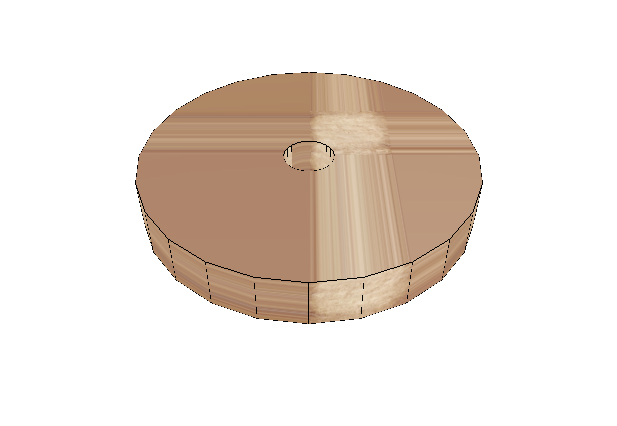
\includegraphics[width=0.6\textwidth]{img/disk.png}
    \caption{Instance of Disk}
    \label{fig:disk}
\end{figure}


\subsubsection{MainStructure Class}

The \texttt{MainStructure} class is responsible for creating the central structure in the Tower of Hanoi game, consisting of a base rectangle and three cylinders. Let's focus on the \texttt{createMainStructure} method, which initializes and positions these components.

\paragraph{Class Structure}

The \texttt{createMainStructure} method is a crucial part of the \texttt{MainStructure} class, where the geometry and material for the main structure are generated. Here's a detailed breakdown of the method:

\begin{lstlisting}[language=JavaScript, caption={JS Class for MainStructure}]

export class MainStructure {
  /**
   * Create the main structure with a base rectangle and three cylinders on top.
   * @param {number} baseWidth - The width of the base rectangle.
   * @param {number} baseDepth - The depth of the base rectangle.
   * @param {number} baseHeight - The height of the base rectangle.
   * @param {number} cylinderRadius - The radius of the cylinders.
   * @param {number} cylinderHeight - The height of the cylinders.
   * @param {string} baseTexturePath - The file path for the base texture image.
   * @param {string} cylinderTexturePath - The file path for the cylinder texture image.
   */
  constructor(baseWidth, baseDepth, baseHeight, cylinderRadius, cylinderHeight, baseTexturePath, cylinderTexturePath) {
    this.baseWidth = baseWidth;
    this.baseDepth = baseDepth;
    this.baseHeight = baseHeight;
    this.cylinderRadius = cylinderRadius;
    this.cylinderHeight = cylinderHeight;
    this.baseTexturePath = baseTexturePath;
    this.cylinderTexturePath = cylinderTexturePath;

    this.createMainStructure();
    this.setDefaultPosition();
  }

  /**
  * Create the geometry and material for the main structure.
  */
  createMainStructure() {
    const loader = new THREE.TextureLoader();

    // Calculate the extended width of the base rectangle
    const extendedWidth = this.baseWidth + 2 * this.cylinderRadius;

    // Calculate the width of each section
    const sectionWidth = this.baseWidth / 3;

    // Load textures
    const baseTexture = loader.load(this.baseTexturePath);
    const cylinderTexture = loader.load(this.cylinderTexturePath);

    // Create the base rectangle geometry with extended sides
    const baseGeometry = new THREE.BoxGeometry(extendedWidth, this.baseHeight, this.baseDepth);
    const baseMaterial = new THREE.MeshBasicMaterial({ map: baseTexture });
    this.baseMesh = new THREE.Mesh(baseGeometry, baseMaterial);
    this.baseMesh.userData.physics = { mass: 1 }; // Set mass for the base

    // Create the cylinder geometry
    const cylinderGeometry = new THREE.CylinderGeometry(this.cylinderRadius, this.cylinderRadius, this.cylinderHeight, 32);
    const cylinderMaterial = new THREE.MeshBasicMaterial({ map: cylinderTexture });

    // Create cylinders and position them in the middle of each section
    this.cylinder1 = new THREE.Mesh(cylinderGeometry, cylinderMaterial);
    this.cylinder1.position.set(-extendedWidth / 2 + this.cylinderRadius + sectionWidth / 2, this.baseHeight / 2 + this.cylinderHeight / 2, 0);
    this.cylinder1.userData.physics = { mass: 1 }; // Set mass for the cylinder

    this.cylinder2 = new THREE.Mesh(cylinderGeometry, cylinderMaterial);
    this.cylinder2.position.set(-extendedWidth / 2 + this.cylinderRadius + sectionWidth + sectionWidth / 2, this.baseHeight / 2 + this.cylinderHeight / 2, 0);
    this.cylinder2.userData.physics = { mass: 1 }; // Set mass for the cylinder

    this.cylinder3 = new THREE.Mesh(cylinderGeometry, cylinderMaterial);
    this.cylinder3.position.set(-extendedWidth / 2 + this.cylinderRadius + 2 * sectionWidth + sectionWidth / 2, this.baseHeight / 2 + this.cylinderHeight / 2, 0);
    this.cylinder3.userData.physics = { mass: 1 }; // Set mass for the cylinder

    // Create a group to hold all the objects
    this.mainStructure = new THREE.Group();
    this.mainStructure.add(this.baseMesh);
    this.mainStructure.add(this.cylinder1);
    this.mainStructure.add(this.cylinder2);
    this.mainStructure.add(this.cylinder3);
  }
// Getter and Setter ...
\end{lstlisting}


\begin{itemize}

\item \textbf{Texture Loading:} The method starts by loading textures for both the base rectangle and the cylinders using the Three.js \texttt{TextureLoader}.

\item \textbf{Base Rectangle Creation:} It creates a base rectangle geometry (\texttt{baseGeometry}) with extended sides to accommodate the cylinders. The material for the base (\texttt{baseMaterial}) is mapped with the loaded base texture.

\item \textbf{Cylinder Creation:} Three cylinders (\texttt{cylinder1}, \texttt{cylinder2}, and \texttt{cylinder3}) are created with appropriate positions. The cylinders are positioned in the middle of each section of the extended base rectangle.

\item \textbf{Physics Properties:} Physics properties (mass) are set for both the base and cylinders, which is useful for physics simulations.

\item \textbf{Grouping Objects:} All created objects, including the base rectangle and cylinders, are grouped together using a Three.js \texttt{Group} (\texttt{mainStructure}).

\end{itemize}

This method ensures that the main structure is created with the correct geometry, material, and positioning, laying the foundation for an integral part of the Tower of Hanoi extended reality game.


\begin{lstlisting}[language=JavaScript, caption={JS Example for MainStructure}]
// Example Usage
const mainStructure = new MainStructure(5, 1, 0.1, 0.05, 0.7, 'path/to/texture_base.jpg', 'path/to/texture_cylinder.jpg')
mainStructure.setPosition(0, 0, 0);
\end{lstlisting}

\begin{figure}[h]
    \centering
    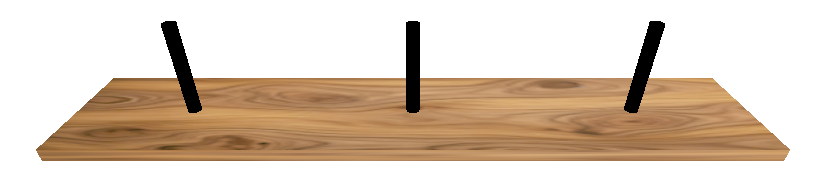
\includegraphics[width=0.6\textwidth]{img/mainStructure.png}
    \caption{Instance of MainStructure}
    \label{fig:mainStructure}
\end{figure}


\subsubsection{Board Class}
To manage the overall presentation and interaction in the Tower of Hanoi game, we implemented the \texttt{Board} class using JavaScript and the Three.js library. The \texttt{Board} class encompasses the visual representation of the game board, including buttons for essential actions and dynamic text to display moves and status.

\paragraph{Class Structure}
The \texttt{Board} class is designed to provide a customizable game board with default parameters for color, height, and width. It includes buttons for actions such as exit, reset, and play/pause, each with associated text for user guidance. The class maintains a count of moves and status information to enhance the gaming experience.

\begin{lstlisting}[language=JavaScript, caption={JS Class for Board}]
export class Board {
  constructor(color = 'grey', boardHeight = 1, boardWidth = 1) {
      this.color = color;
      this.boardHeight = boardHeight;
      this.boardWidth = boardWidth;
      this.moves = 0; // Initialize moves
      this.status = 'valid'; // Initialize status

      // Create the board geometry and material
      const boardGeometry = new THREE.PlaneGeometry(this.boardWidth, this.boardHeight);
      const boardMaterial = new THREE.MeshBasicMaterial({ color: this.color, side: THREE.DoubleSide });
      this.board = new THREE.Mesh(boardGeometry, boardMaterial);

      // Create buttons
      this.createButtons();
      this.createText();
  }

  createButtons() {
      // Define button dimensions
      const buttonWidth = 0.6;
      const buttonHeight = 0.2;
      const buttonDepth = 0.1;
      const buttonGeometry = new THREE.BoxGeometry(buttonWidth, buttonHeight, buttonDepth);

      // Example: Exit Button
      const exitMaterial = new THREE.MeshBasicMaterial({ color: 0xff0000 }); // red color
      this.exit = new THREE.Mesh(buttonGeometry, exitMaterial);
      this.exit.position.set(-this.boardWidth / 2 + buttonWidth, this.boardHeight / 2 - buttonHeight, 0.1);
      

      // Example: Reset Button
      const resetMaterial = new THREE.MeshBasicMaterial({ color: 0x0000ff }); // blue color
      this.reset = new THREE.Mesh(buttonGeometry, resetMaterial);
      this.reset.position.set(-this.boardWidth / 2 + 3 * buttonWidth, this.boardHeight / 2 - buttonHeight, 0.1);
      

      const playMaterial = new THREE.MeshBasicMaterial({ color: 0x0000ff }); // blue color
      this.play = new THREE.Mesh(buttonGeometry, playMaterial);
      this.play.position.set(-this.boardWidth / 2 + 5 * buttonWidth, this.boardHeight / 2 - buttonHeight, 0.1);

      const loader = new FontLoader();
      loader.load('./assets/helvetiker_regular.typeface.json', (font)=>{
          const textOptions = {
              font: font,
              size: 0.05,
              height: 0.05,
          };
      // Create text geometry for each button
      const exitTextGeometry = new TextGeometry('Exit', textOptions);
      const resetTextGeometry = new TextGeometry('Reset', textOptions);
      const play_pauseTextGeometry = new TextGeometry('Play/Pause', textOptions);

      // Create meshes for the text
      const textMaterial = new THREE.MeshBasicMaterial({ color: 0xffffff });
      const exitText = new THREE.Mesh(exitTextGeometry, textMaterial);
      const resetText = new THREE.Mesh(resetTextGeometry, textMaterial);
      const playPauseText = new THREE.Mesh(play_pauseTextGeometry, textMaterial);

      // Position the text on the buttons
      exitText.position.set(-0.1, -0.05, 0.05); // Adjust these values as needed
      resetText.position.set(-0.1, -0.05, 0.05);
      playPauseText.position.set(-0.1, -0.05, 0.05);

      // Add the text to the buttons
      console.log(this.exit)
      this.exit.add(exitText);
      this.reset.add(resetText);
      this.play.add(playPauseText);
      });

      this.board.add(this.exit);
      this.board.add(this.reset);
      this.board.add(this.play);
  }

  createText() {
        const loader = new FontLoader();
        loader.load('./assets/helvetiker_regular.typeface.json', (font) => {
          this.font = font; // Store the font for later use
          this.updateMovesAndStatus(0, 'valid'); // Initial text setup
      });
    }

    updateMovesAndStatus(moves, invalid) {
      this.moves = moves;
        if (invalid == true){
          this.status = 'invalid';
        }
        else{
          this.status = 'valid';
        }

      const textOptions = {
          font: this.font,
          size: 0.3,
          height: 0.05,
      };

      // Update moves text
      if (this.movesText) this.board.remove(this.movesText); // Remove old text
      const movesTextGeometry = new TextGeometry('Moves: ' + this.moves, textOptions);
      const movesTextMaterial = new THREE.MeshBasicMaterial({ color: 0xffffff });
      this.movesText = new THREE.Mesh(movesTextGeometry, movesTextMaterial);
      this.movesText.position.set(-this.boardHeight / 2, 0, 0);
      this.board.add(this.movesText);

      // Update status text
      if (this.statusText) this.board.remove(this.statusText); // Remove old text
      const statusTextGeometry = new TextGeometry('Status: ' + this.status, textOptions);
      const statusTextMaterial = new THREE.MeshBasicMaterial({ color: 0xffffff });
      this.statusText = new THREE.Mesh(statusTextGeometry, statusTextMaterial);
      this.statusText.position.set(-this.boardHeight / 2, -this.boardWidth / 4, 0);
      this.board.add(this.statusText);
  }
}
\end{lstlisting}

\paragraph{Button and Text Creation}
The \texttt{createButtons} method generates interactive buttons on the board, such as exit, reset, and play/pause. These buttons include 3D geometries with associated materials for visual appeal. Text labels are added to the buttons using the Three.js library's capabilities.

\paragraph{Text Display and Updates}
The \texttt{createText} method initializes the font for later use in displaying text on the board. The \texttt{updateMovesAndStatus} method dynamically updates and displays the move count and game status. This interactive text provides valuable feedback to the player during gameplay.

\begin{lstlisting}[language=JavaScript, caption={JS Example for Board}]
// Example Usage
const gameBoard = new Board('blue', 2, 2);
gameBoard.updateMovesAndStatus(5, false);
\end{lstlisting}

In this example, a game board is instantiated with specific parameters, and the moves and status are updated during gameplay. The \texttt{Board} class enhances the Tower of Hanoi game interface, combining visual elements and interactivity for an engaging user experience.

\begin{figure}[h]
    \centering
    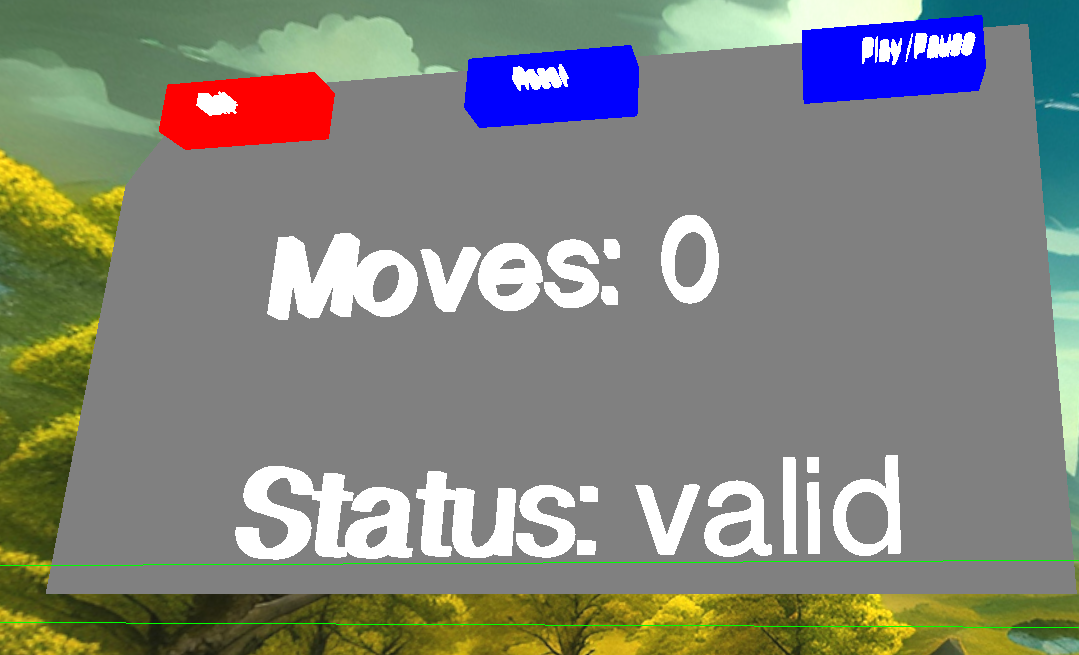
\includegraphics[width=0.6\textwidth]{img/board.png}
    \caption{Instance of Board}
    \label{fig:board}
\end{figure}


\subsection{3D Background Environment}

To enhance the immersive quality of the Tower of Hanoi game, we implemented a 3D background environment using the GLTFLoader in Three.js. This addition introduces an extra layer to the scene, providing a sense of depth and presence for a more engaging visual experience.

\begin{lstlisting}[language=JavaScript, caption={JS Code for Including 3D Background}]
setUpBackground() {
    const loader = new GLTFLoader();
    loader.load('../../assets/models/back.glb', 
        (gltf) => {
            const model = gltf.scene;
            model.position.z = 1;
            this.scene.add(model);
        },
        (xhr) => {
            // Progress callback (optional)
            // console.log((xhr.loaded / xhr.total * 100) + '% loaded');
        },
        (error) => {
            console.error('Error loading the model:', error);
        }
    );
}
\end{lstlisting}

\paragraph{Code Explanation:}

\begin{itemize}
    \item \textbf{Loader Initialization:} An instance of the GLTFLoader is created, which is a loader specifically designed for loading models in the glTF format, a popular format for 3D models.

    \item \textbf{Model Loading:} The loader loads the 3D model from the specified file path ('../../assets/models/back.glb'). Upon successful loading, the provided callback function is executed, receiving a glTF object (\texttt{gltf}).

    \item \textbf{Scene Placement:} The 3D model is retrieved from the glTF object (\texttt{gltf.scene}). The model's position is set to have a positive z-coordinate (\texttt{model.position.z = 1}), placing it slightly in front of the camera in the scene.

    \item \textbf{Adding to Scene:} The model is added to the main scene (\texttt{this.scene}), integrating it as part of the overall 3D environment.

    \item \textbf{Progress Callback (Optional):} During the loading process, a progress callback is provided (commented out in this case). It can be used to track the loading progress if needed.

    \item \textbf{Error Handling:} If there is an error during the loading process, an error message is logged to the console (\texttt{console.error('Error loading the model:', error)}).
\end{itemize}

This code segment ensures that the 3D background model is loaded and positioned appropriately within the Three.js scene, contributing to the immersive quality of the Tower of Hanoi game.

Here is a part of the background:
\begin{figure}[h]
    \centering
    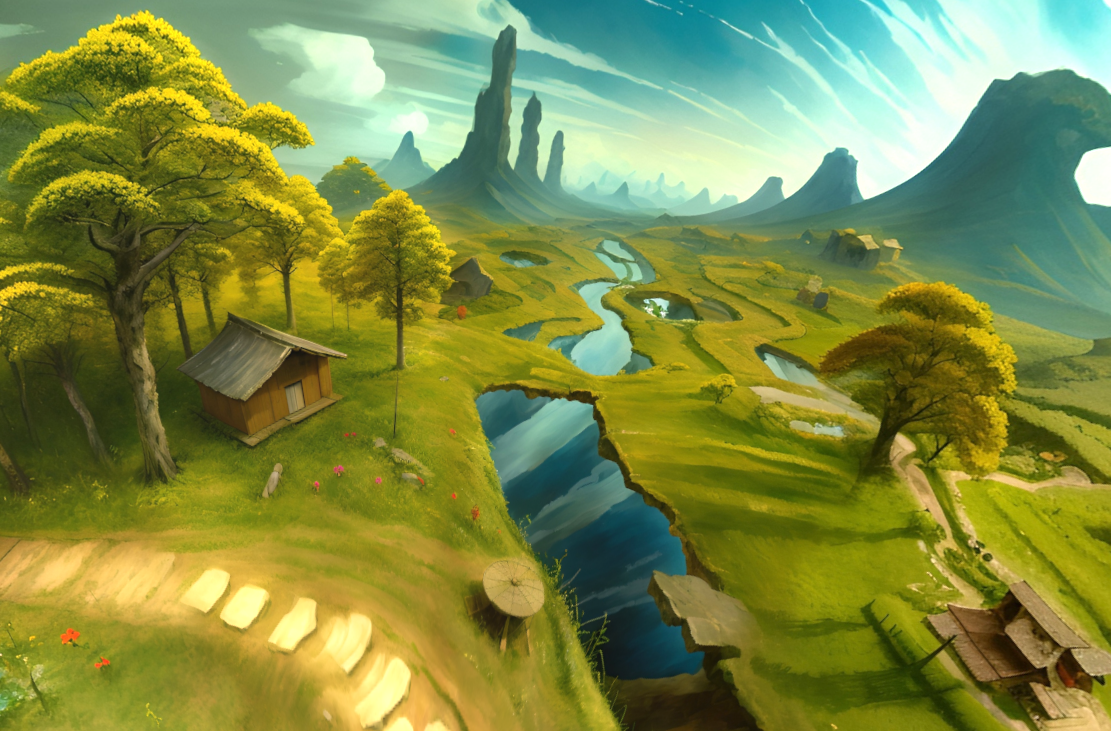
\includegraphics[width=0.6\textwidth]{img/back.png}
    \caption{Part of the 3D Background}
    \label{fig:back}
\end{figure}


\subsection{Background Music}

To enrich the gaming experience, we introduced a carefully curated background soundtrack to the Tower of Hanoi extended reality game. The background music enhances the immersive atmosphere, providing players with a multi-sensory experience that complements the gameplay.

\begin{lstlisting}[language=JavaScript, caption={JS code for adding Audio}]
setUpAudio() {
    // Create an audio listener attached to the camera
    const listener = new THREE.AudioListener();
    this.camera.add(listener);

    // Create a global audio object
    const audio = new THREE.Audio(listener);

    // Create an AudioLoader
    const audioLoader = new THREE.AudioLoader();

    // Load the soundtrack
    audioLoader.load('../../assets/sakura.mp3', (buffer) => {
        // Set the audio buffer and configure playback properties
        audio.setBuffer(buffer);
        audio.setLoop(true); // Loop the soundtrack
        audio.setVolume(2); // Adjust the volume (2 times the normal volume)
        audio.play(); // Start playing the soundtrack
    });
}
\end{lstlisting}

\paragraph{Code Explanation:}

\begin{itemize}
    \item \textbf{Audio Listener Creation:} An audio listener is created using \texttt{THREE.AudioListener()}, and it is attached to the camera to ensure that the audio is spatialized based on the camera's position.

    \item \textbf{Global Audio Object:} A global audio object (\texttt{audio}) is created using the audio listener.

    \item \textbf{AudioLoader Initialization:} An \texttt{AudioLoader} is instantiated to load the soundtrack asynchronously.

    \item \textbf{Soundtrack Loading:} The \texttt{audioLoader.load()} method loads the soundtrack from the specified file path ('../../assets/sakura.mp3'). Upon successful loading, the provided callback function is executed, receiving an \texttt{AudioBuffer} (\texttt{buffer}).

    \item \textbf{Audio Configuration:} The audio buffer is set for the \texttt{audio} object, and playback properties are configured. The soundtrack is set to loop indefinitely, and its volume is adjusted (2 times the normal volume).

    \item \textbf{Start Playback:} The \texttt{audio.play()} method is called to start playing the background soundtrack.

\end{itemize}

This code segment ensures the seamless integration of background music into the Tower of Hanoi extended reality game, contributing to a more immersive and enjoyable gaming experience.

\newpage
\subsection{Final Environment}

\begin{figure}[h]
    \centering
    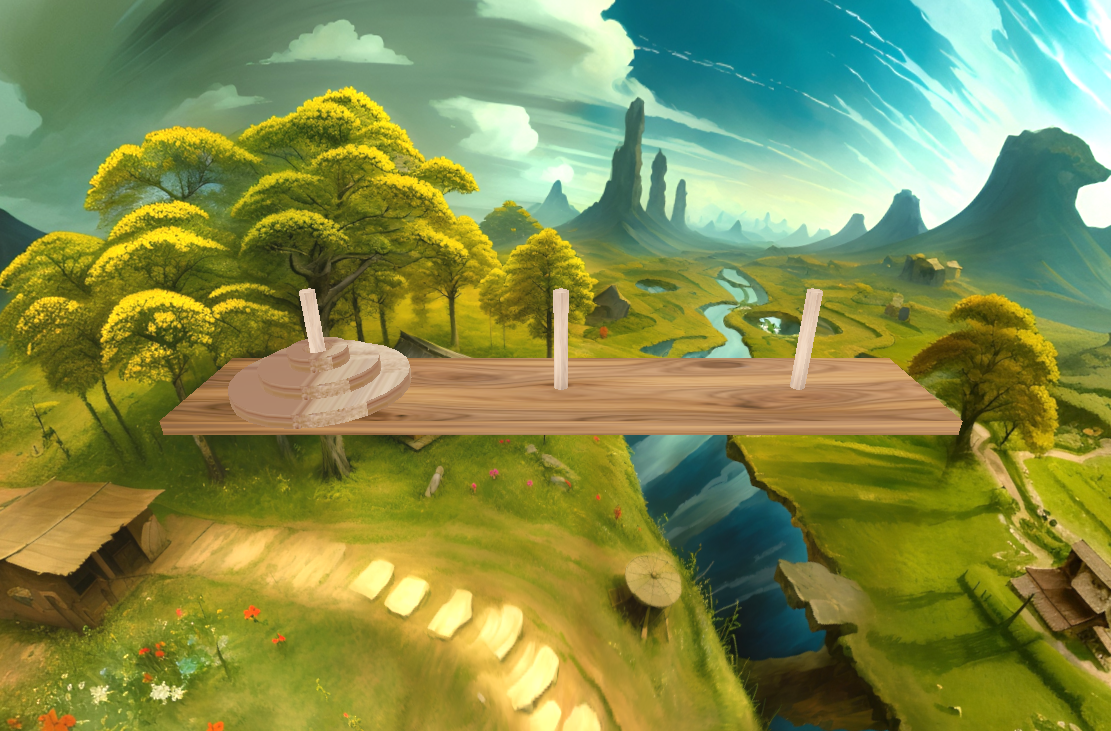
\includegraphics[width=1\textwidth]{img/result.png}
    \caption{Final Environment with 3 Disks, Main Structure, Background, and Music.}
    \label{fig:final_environment}
\end{figure}

\section{Physics Implementation}
\subsection{Drag and Drop Implementation with DragControls}

To enhance user interaction, we implemented the drag and drop functionality using DragControls in Three.js. This feature allows users to select and move game objects seamlessly within the 3D environment.

\begin{lstlisting}[language=JavaScript, caption={JS Class for Drag Control}]
export class DraggablesManager {
  constructor(objects, camera, renderer, scene) {
    this.objects = objects;
    this.dragControls = new DragControls(this.objects, camera, renderer.domElement);

    //this.dragControls.addEventListener('hoveron', this.onHoverOn.bind(this));
    //this.dragControls.addEventListener('hoveroff', this.onHoverOff.bind(this));

  }

  addObject(object) {
    this.objects.push(object);
    this.dragControls.setObjects(this.objects);
  }

  onHoverOn(event) {
    // Add your logic when hovering on an object
    const hoveredObject = event.object;
    console.log('Hovered on:', hoveredObject);
  }

  onHoverOff(event) {
    // Add your logic when hovering off an object
    const unhoveredObject = event.object;
    console.log('Hovered off:', unhoveredObject);
  }
}
\end{lstlisting}

\paragraph{Code Explanation:}

\begin{itemize}
    \item \textbf{DragControls Initialization:} We initialized the DragControls to enable the drag and drop functionality. This included creating an instance of DragControls, associating it with the camera and the array of draggable objects.

    \item \textbf{Event Handling:} We set up event listeners to handle the start, drag, and end events triggered by DragControls. These events enabled us to update the position of the dragged object during interaction.

    \item \textbf{Selectable Objects:} We defined the array of selectable objects to include the disks in the Tower of Hanoi game. These objects became draggable and responsive to user input.

\end{itemize}

This implementation provides an intuitive way for users to interact with the Tower of Hanoi game by selecting and moving objects using drag and drop functionality.


\section{Rule Implementation}

In the Tower of Hanoi game, the implementation of rules is crucial for ensuring a challenging and engaging experience. One of the key functions responsible for enforcing game rules is the \texttt{checkCollisions} function.

\subsection{Collision Detection}

The \texttt{checkCollisions} function is responsible for detecting collisions between disks during gameplay. It utilizes the bounding box technique to determine if any two disks intersect. The bounding box for each disk is updated based on its current position and orientation in the 3D space.

\begin{lstlisting}[language=JavaScript, caption={Collision Detection Function}]
function checkCollisions() {
    scene.disk1BB.copy(scene.disks[0].mesh.geometry.boundingBox).applyMatrix4(scene.disks[0].mesh.matrixWorld);
    scene.disk2BB.copy(scene.disks[1].mesh.geometry.boundingBox).applyMatrix4(scene.disks[1].mesh.matrixWorld);
    scene.disk3BB.copy(scene.disks[2].mesh.geometry.boundingBox).applyMatrix4(scene.disks[2].mesh.matrixWorld);

    // Check for collisions between Disk 1 and Disk 2
    if (scene.disk1BB.intersectsBox(scene.disk2BB)) {
        if (scene.disks[0].mesh.position.y > scene.disks[1].mesh.position.y) {
            Invalid = true;
        }
    }

    // Check for collisions between Disk 1 and Disk 3
    if (scene.disk1BB.intersectsBox(scene.disk3BB)) {
        if (scene.disks[0].mesh.position.y > scene.disks[2].mesh.position.y) {
            Invalid = true;
        }
    }
    // Check for collisions between Disk 2 and Disk 3
    if (scene.disk2BB.intersectsBox(scene.disk3BB)) {
        if (scene.disks[1].mesh.position.y > scene.disks[2].mesh.position.y) {
            Invalid = true;
        }
    }
}
\end{lstlisting}

In the code snippet above, the function checks for collisions between each pair of disks (Disk 1 and Disk 2, Disk 1 and Disk 3, Disk 2 and Disk 3) and updates the game state accordingly.

This collision detection mechanism adds a layer of complexity to the Tower of Hanoi game, requiring players to adhere to the rules and make strategic moves to successfully complete the puzzle.


\subsection{Drag-and-Drop Interaction}

Enabling a seamless drag-and-drop interaction for the Tower of Hanoi game enhances the user experience and allows players to make strategic moves. The implementation involves utilizing event listeners and controls provided by the Three.js library.

\begin{lstlisting}[language=JavaScript, caption={Drag-and-Drop Interaction}]
    scene.controls.addEventListener( 'drag', function(event){
        if (selected?.body.getCollisionFlags() === 2) {
            const { x, y } = pointer
            const speed = 0.03
            const movementX = (x - prev.x) * speed
            const movementZ = (y - prev.y) * -speed
            selected.position.x += movementX
            selected.position.z += movementZ
            selected.body.needUpdate = true
            prev = { x, y }
        }
        selectedObject = event.object
        render();
    } );

document.addEventListener( 'pointermove', onPointerMove );
document.addEventListener( 'pointerdown', onPointerDown );

scene.controls.addEventListener('dragstart', function (event) {
    // Disable orbit control during drag
    makingMove = true;
    orbitControls.enabled = false;
    selectedObject = event.object;

    // Check for intersecting disks during drag start
    const intersects_disks = raycaster.intersectObjects( scene.disks_mashes, true );
    if ( intersects_disks.length > 0 ) {
        intersects_disks[0].object.material.color.set( 0xffb3b3 ); // Change color of selected object
        let disk_onTop = hasDisksOnTop(intersects_disks[0].object,scene.disks_mashes);
        console.log("disk on top variable: ",disk_onTop);

        if(disk_onTop === false){
            selected = intersects_disks[0].object;
            console.log("selected: ",selected.body.getCollisionFlags());
            selected.body.setCollisionFlags(2); // Set collision flag for the dragged disk
        }
    }
});

scene.controls.addEventListener('dragend', function (event) {
    // Enable orbit control after drag ends
    makingMove = false;
    orbitControls.enabled = true;
    const selectedObject = event.object;

    // Check if the dragged object is a disk
    if (selectedObject.body.getCollisionFlags() === 2){
        movesMade +=1; // Increment move count
    }

    selectedObject.material.color.setHex( CURRENTCOLOR );
    selectedObject.body.setCollisionFlags(0); // Reset collision flag

    // When the object is dropped, check if it is on the table
    // If on the table, set the collision flag to 1 (static)
    selectedObject.body.on.collision((otherObject, event) => {
        if (otherObject.name === 'table') selectedObject.body.setCollisionFlags(1);
    })

    selected = null; // Reset selected object
});
\end{lstlisting}

In the provided code snippet, the drag-and-drop interaction is handled through event listeners and controls. The drag, dragstart, and dragend events are utilized to manage the state of the interaction, enable/disable orbit control, and update relevant parameters.

The drag-and-drop feature enhances player control and adds an interactive layer to the Tower of Hanoi game.

\subsection{Rendering and Game State Update}

The rendering process in the Tower of Hanoi game plays a crucial role in updating the game state, including the move count and game status. The \texttt{render} function is responsible for orchestrating these updates, ensuring a smooth and responsive gaming experience.

\begin{lstlisting}[language=JavaScript, caption={Rendering and Game State Update}]
function render(event) {
    // Check for collisions if not in the process of making a move
    if (makingMove == false) {
        checkCollisions();
    }

    // Update physics simulation
    physics.update(clock.getDelta() * 1000);
    physics.updateDebugger();

    // Render the scene
    scene.renderer.render(scene.scene, scene.camera);

    // Update the game board with the latest move count and status
    scene.gameBoard.updateMovesAndStatus(movesMade, Invalid);
}

// Initial update of the game board state
scene.gameBoard.updateMovesAndStatus(movesMade, Invalid);
\end{lstlisting}

In the code snippet above, the \texttt{render} function is described as the central hub for updating the game state during the rendering process. It checks for collisions, updates the physics simulation, renders the scene, and ensures that the game board reflects the latest move count and status.

This integration of rendering and game state update contributes to a responsive and visually informative Tower of Hanoi gaming experience.



\end{document}
